This chapter presents the user interfaces of our application, showcasing key designs related to meaningful use cases. Each interface is tailored to specific functionalities and workflows, reflecting how users interact with the system to accomplish their goals. By illustrating these interfaces, we aim to provide a clear understanding of the application's usability, layout, and design principles.

In the RASD, interfaces for login and the main pages of the application were introduced. In this document, we extend this by presenting additional interfaces associated with other important use cases, further demonstrating how the system supports user needs in a seamless and intuitive manner.

\section{Sign Up [UC1]}
\label{sec:UI1_sign_up}%

The first interface is tailored for students, requiring inputs for email, password, first name, last name, and username. The "Accept \& Join" button finalizes the sign-up.

\begin{figure}[H]
    \centering
    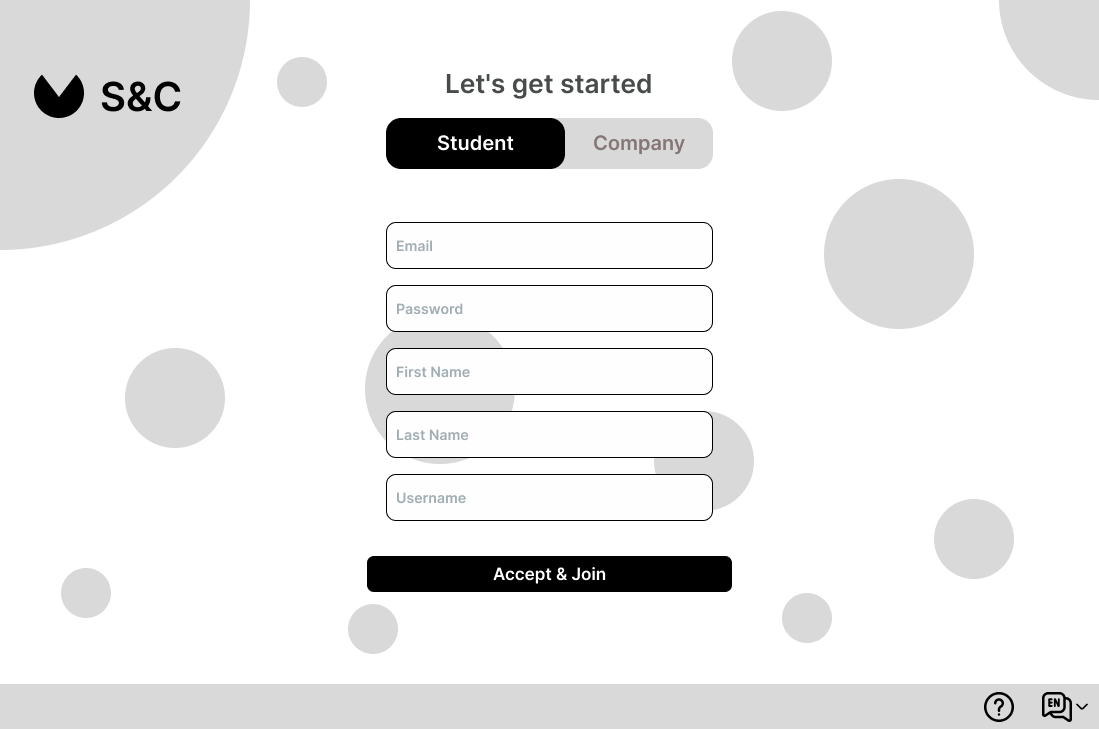
\includegraphics[width=0.75\linewidth]{DD/Images/UI/Signin_Student.png}
    \caption{Sign Up Student.}
    \label{fig:signup_stud_ui}
\end{figure}

The second interface allows company representatives to create accounts by filling out fields for email, password, name, VAT name, and username. The "Accept \& Join" button completes the registration process.

\begin{figure}[H]
    \centering
    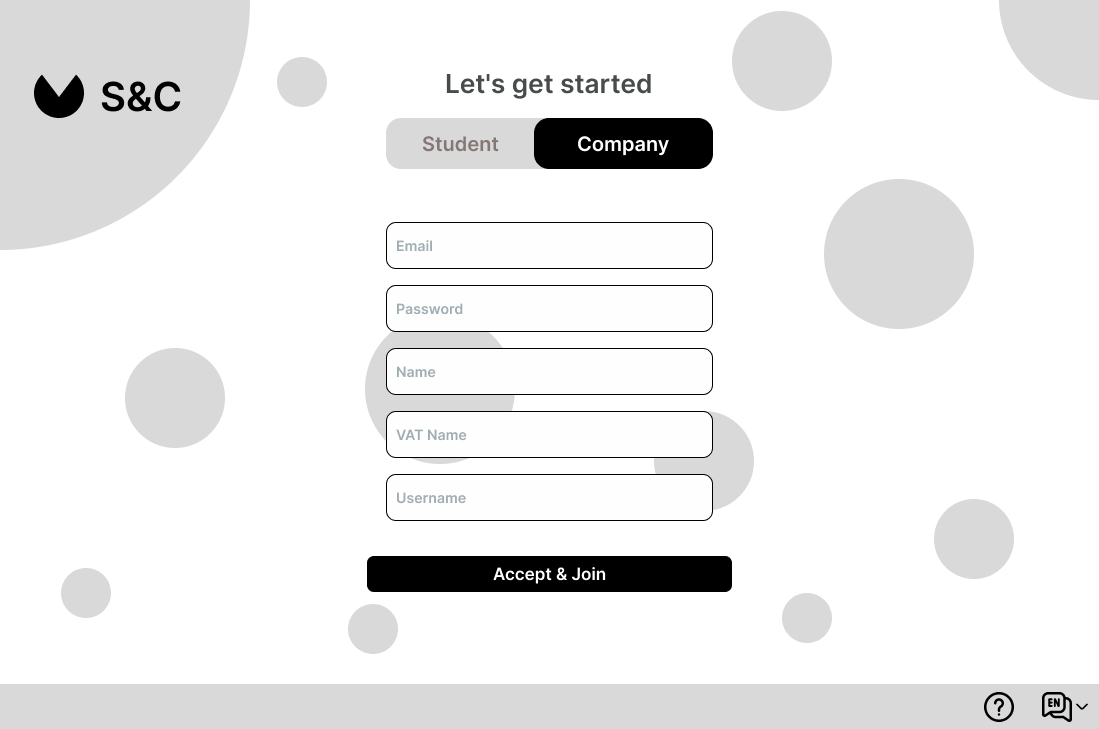
\includegraphics[width=0.75\linewidth]{DD/Images/UI/Signin_Company.png}
    \caption{Sign Up Company.}
    \label{fig:signup_comp_ui}
\end{figure}

A toggle at the top lets users easily switch between the Student and Company sign-up forms.

\newpage

\section{Insert an enhanced Internship Insertion [UC3]}
\label{sec:UI2_enhanced_intern}%


\textbf{\autoref{fig:post_intern_ui}:} Initial Postage

The first phase represents the initial "Post a New Internship Insertion" form. This interface is displayed when the user clicks the "Post" button on the homepage. The form contains fields for the internship's position name, location, duration, start date, and description, allowing the user to provide all necessary details.

\begin{figure}[H]
    \centering
    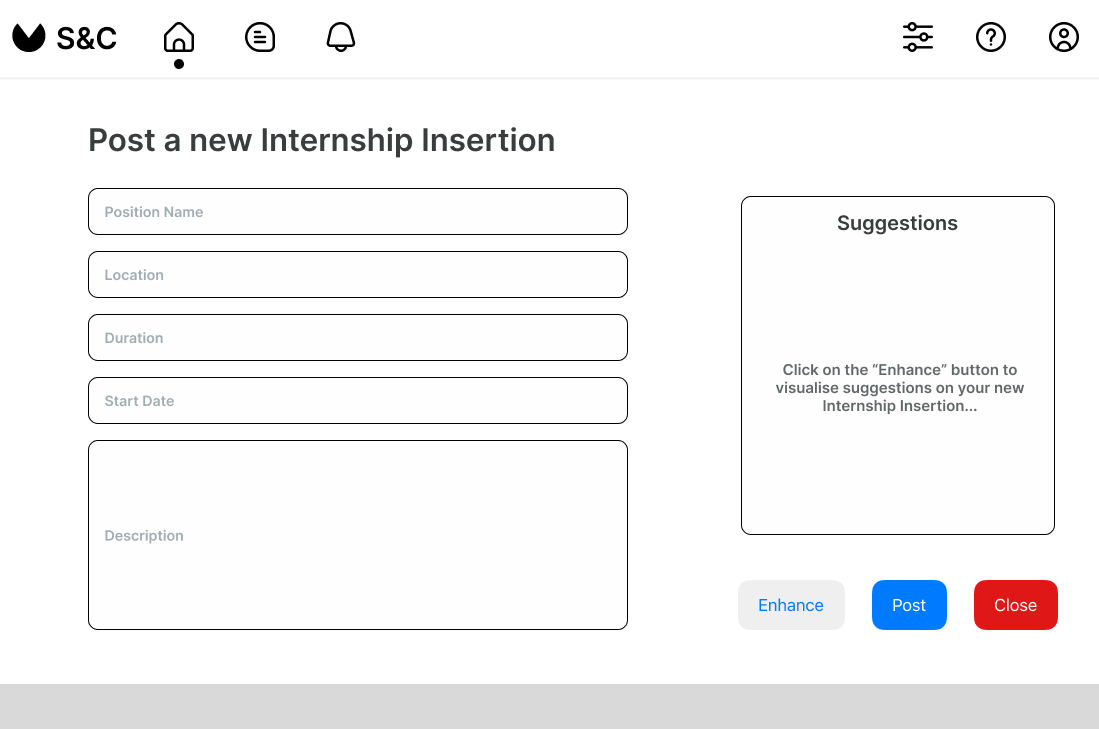
\includegraphics[width=0.75\linewidth]{DD/Images/UI/Postpage.png}
    \caption{Post a New Internship.}
    \label{fig:post_intern_ui}
\end{figure}

\textbf{\autoref{fig:post_intern_fill_ui}:} Filled Form

In the second phase, the form is shown with all fields filled in by the user. The system is now ready to process or enhance the insertion based on the provided information.

\begin{figure}[H]
    \centering
    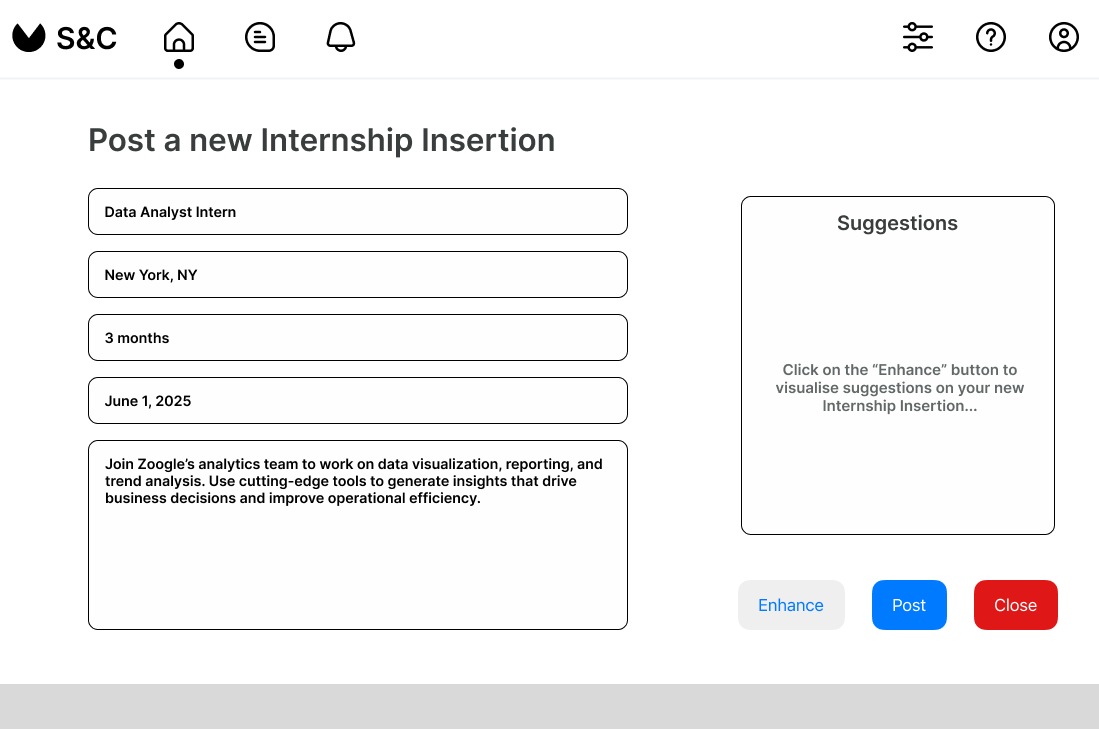
\includegraphics[width=0.75\linewidth]{DD/Images/UI/Postpage_filledForm.png}
    \caption{Post a New Internship (filled).}
    \label{fig:post_intern_fill_ui}
\end{figure}


\textbf{\autoref{fig:post_intern_enhance_ui}:} Enhanced Suggestions

The final phase is displayed after the user clicks the "Enhance" button. The system processes the input data and provides suggestions on the right panel to improve the internship insertion. These suggestions may add more specific details to the description to make the posting more appealing and clear.

\begin{figure}[H]
    \centering
    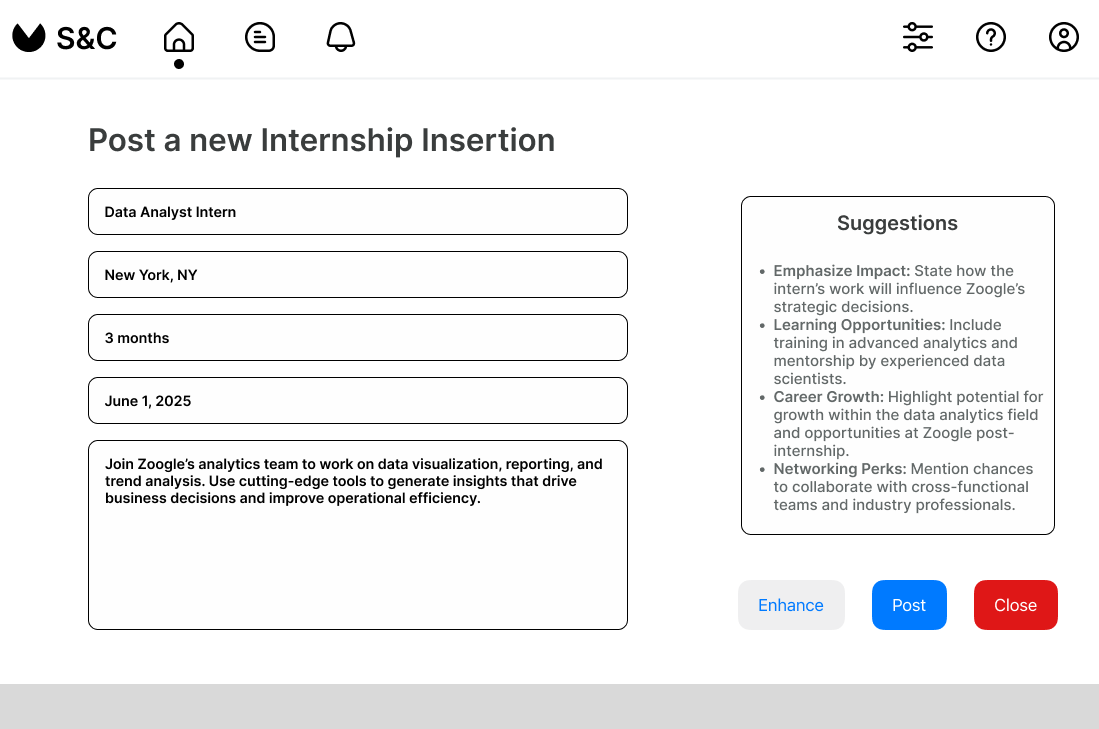
\includegraphics[width=0.75\linewidth]{DD/Images/UI/Postpage_filledForm_enhance.png}
    \caption{Suggestions on the Internship Post.}
    \label{fig:post_intern_enhance_ui}
\end{figure}



\section{Enhance CV [UC4]}
\label{sec:UI3_enhanced_CV}%

\textbf{\autoref{fig:myprofile_page_ui}:} Viewing the Profile

The first figure represents the profile page of a student within the application. This page displays the student's personal information, such as:

Name, Date of Birth, City, University, Mobile Number, Email and Password, and a section for the uploaded CV file.
The student has the option to upload or enhance his CV using the respective buttons.

\begin{figure}[H]
    \centering
    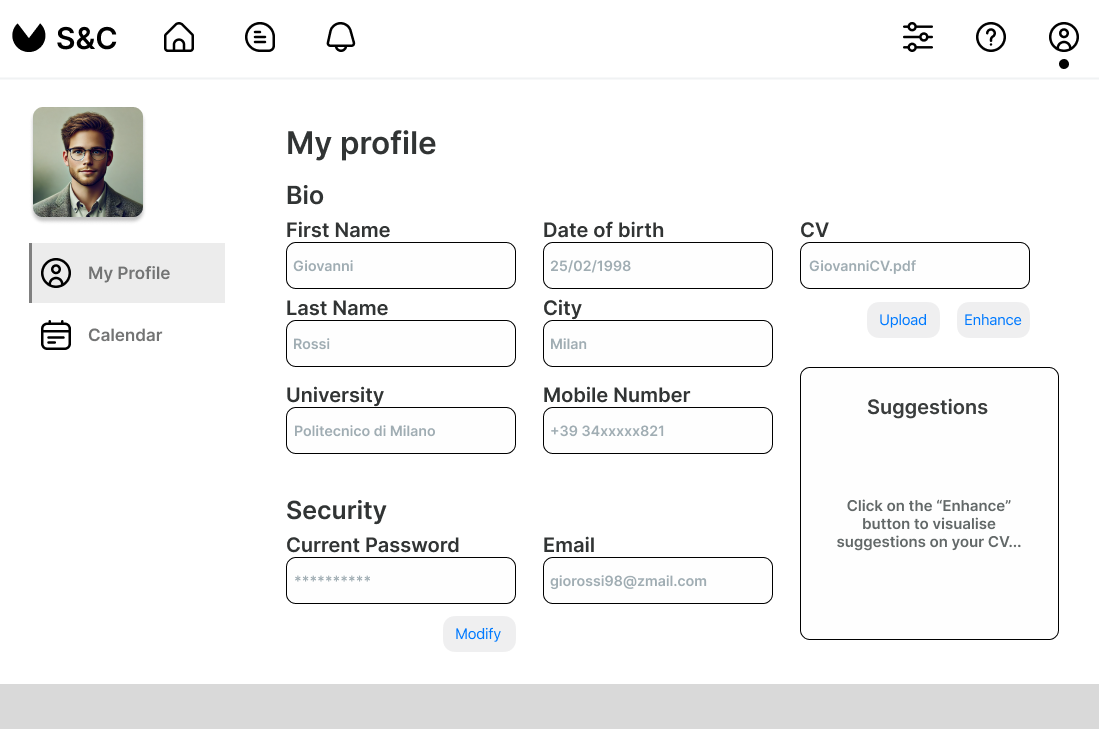
\includegraphics[width=0.75\linewidth]{DD/Images/UI/MyProfile.png}
    \caption{MyProfile page.}
    \label{fig:myprofile_page_ui}
\end{figure}

\textbf{\autoref{fig:myprofile_page_enhance_ui}:} Enhancing the CV

The second figure is the result of clicking the Enhance button. The system processes the uploaded CV and provides tailored suggestions in the "Suggestions" section to improve the CV. Examples include adding specific skills, quantifying achievements, or including relevant certifications.

\begin{figure}[H]
    \centering
    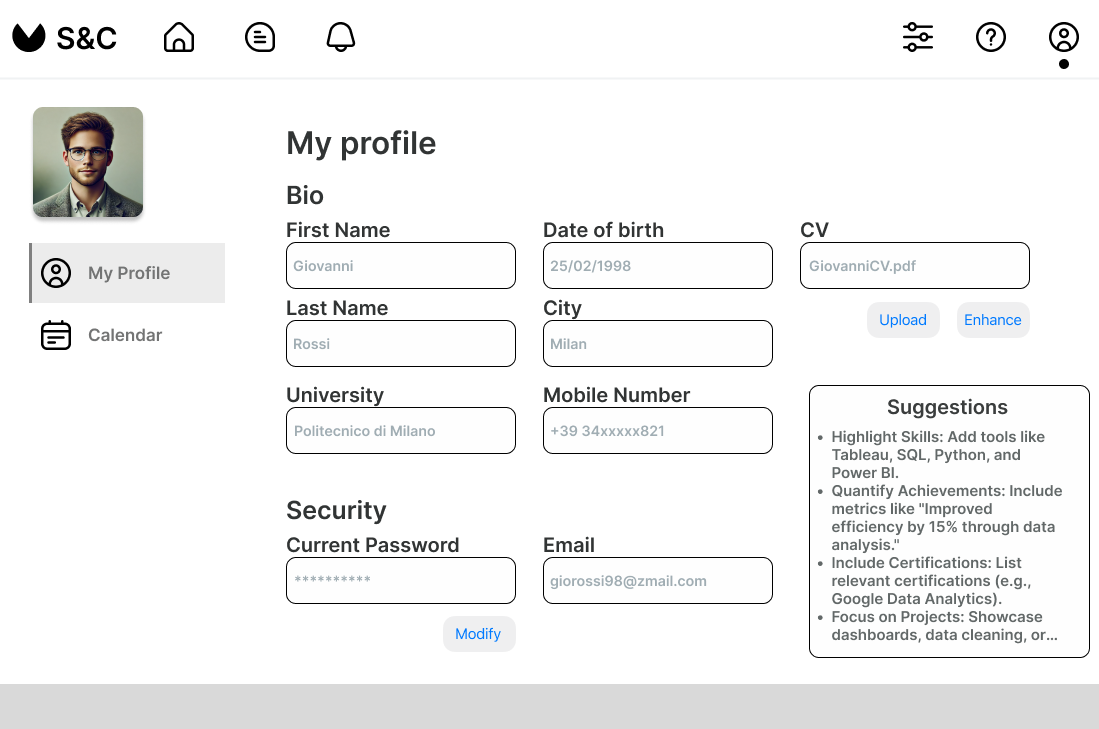
\includegraphics[width=0.75\linewidth]{DD/Images/UI/MyProfile_enhanceCV.png}
    \caption{MyProfile page (enhance).}
    \label{fig:myprofile_page_enhance_ui}
\end{figure}

\textbf{Modifying the CV}

If the student decides to act on the suggestions, they need to modify the CV file externally using their preferred editing tools. Once updated, the student can re-upload the revised CV using the Upload button on the same profile page.

This flow ensures the CV remains user-controlled while benefiting from AI-driven enhancement suggestions provided by the system.

\newpage

\section{Submit a Feedback [UC5]}
\label{sec:UI4_submit_feedback}%

\textbf{\autoref{fig:recomm_insertion_ui}:} Viewing a Recommendation

The first image represents the system’s recommendation for an internship insertion, tailored based on the analysis of the user. It includes key details:
Position Title, Location, Duration, Start Date and a Description.

The user can click the "Apply" button to proceed (as explained on the [UC7]) or close the recommendation by clicking the exit button (X) in the top-right corner.

\begin{figure}[H]
    \centering
    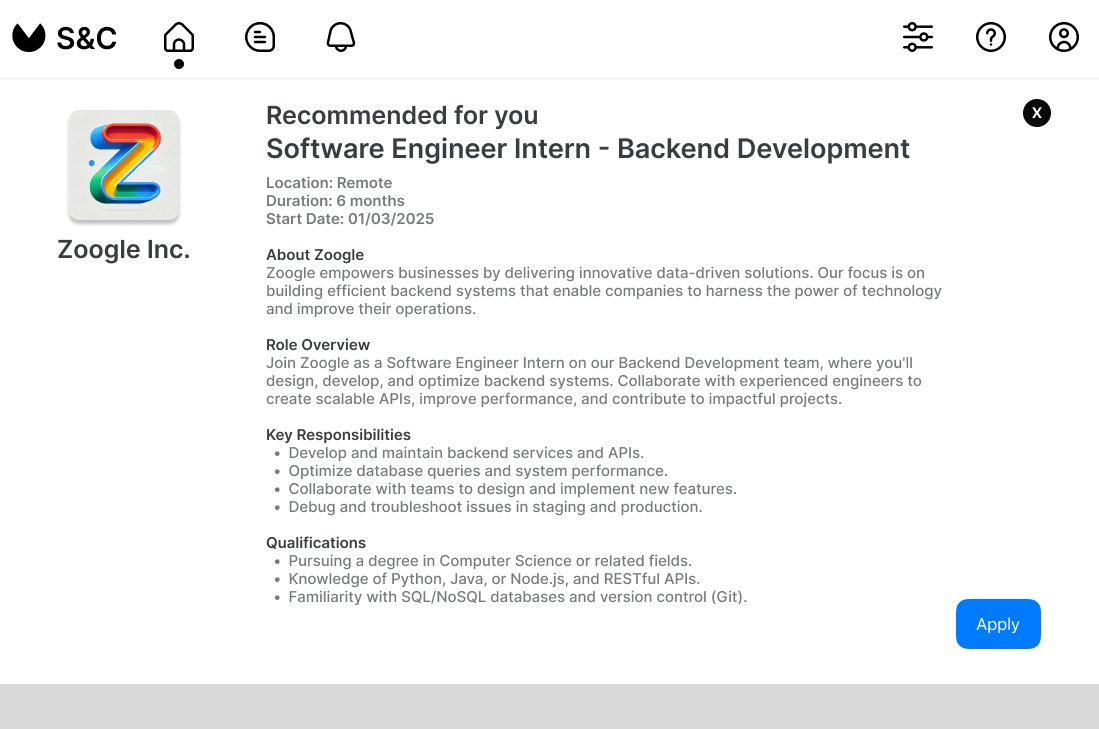
\includegraphics[width=0.75\linewidth]{DD/Images/UI/recommInsertion.png}
    \caption{Recommended Insertion.}
    \label{fig:recomm_insertion_ui}
\end{figure}

\newpage

\textbf{\autoref{fig:feedback_ui}:} Providing Feedback

The second image is displayed when the user clicks the exit button (X) to close the recommendation. A pop-up asks the user to submit feedback on the recommendation, including:

\begin{itemize}
    \item 
Rating: A 5-star rating system to evaluate the relevance or quality of the recommendation.
    \item 
Comments: A text box where the user can provide additional feedback, such as what they liked or what could be improved.
\end{itemize}

The "Submit" button sends the feedback to the system, helping refine future recommendations.

\begin{figure}[H]
    \centering
    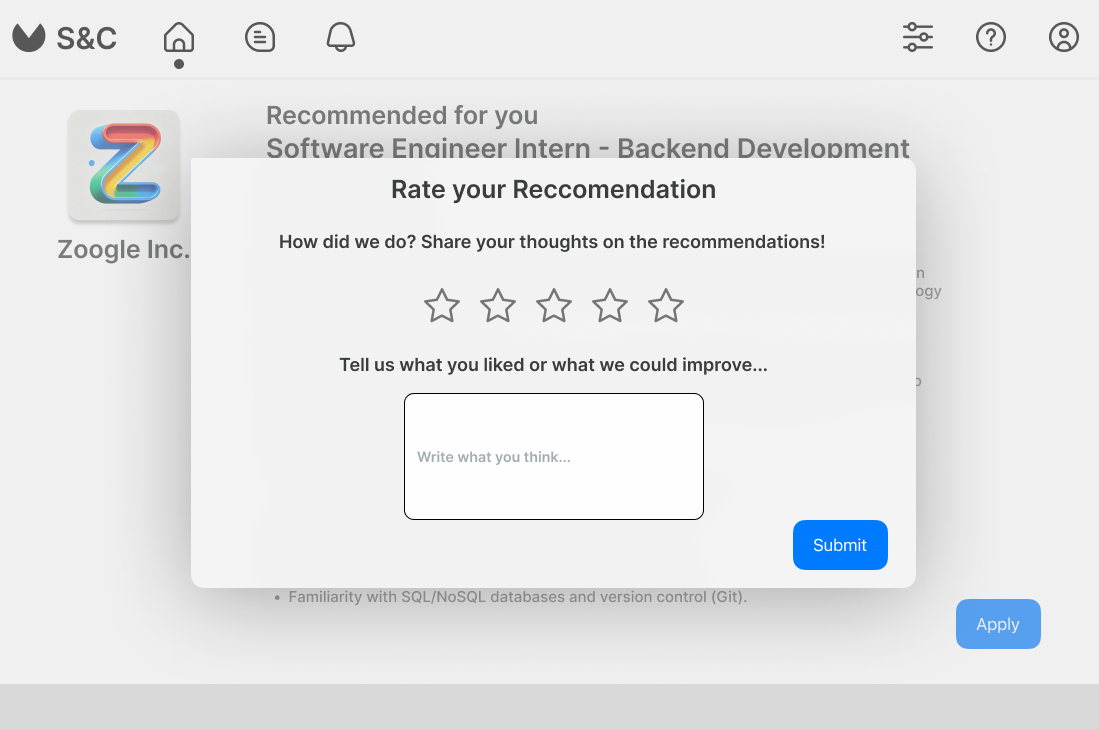
\includegraphics[width=0.75\linewidth]{DD/Images/UI/recommInsertionFeedback.png}
    \caption{Ask for a Feedback.}
    \label{fig:feedback_ui}
\end{figure}

\newpage

\section{Accept a Candidate [UC8]}
\label{sec:UI5_accept_candidate}

\textbf{\autoref{fig:insertions_ui}:} View Internship Insertions

The first image represents the list of all internship insertions posted by the company. Each insertion is displayed with its title and location, allowing the company to select the relevant internship they wish to manage.

\begin{figure}[H]
    \centering
    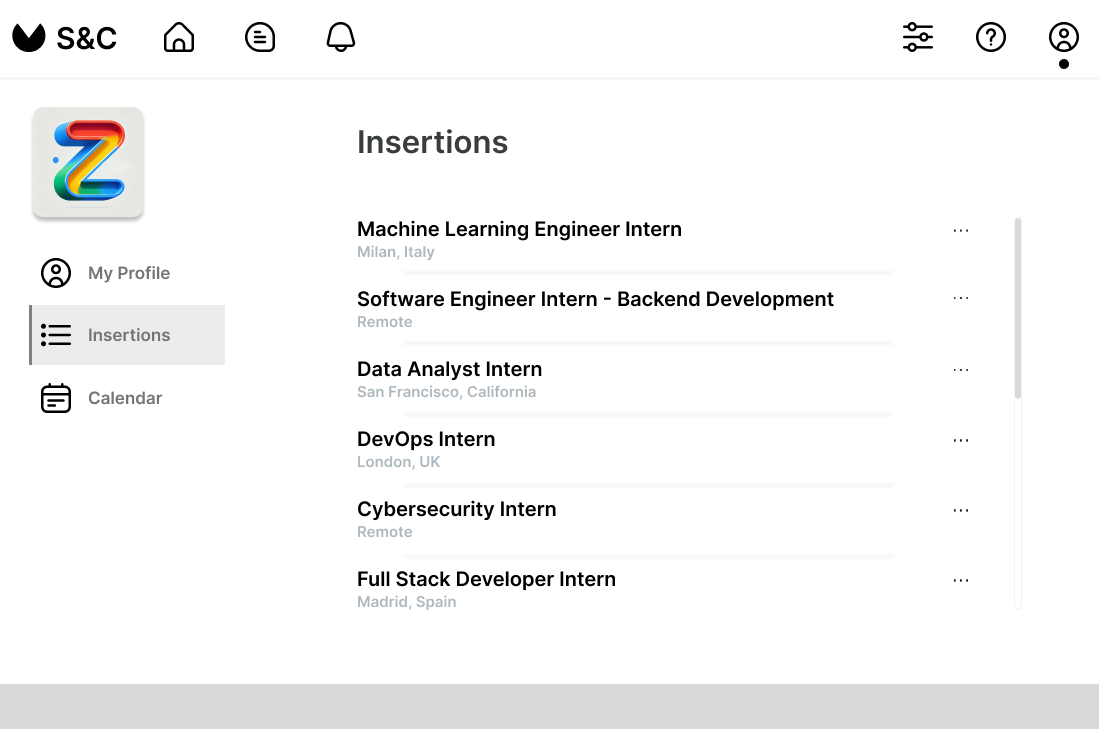
\includegraphics[width=0.75\linewidth]{DD/Images/UI/Insertions.png}
    \caption{Insertions posted.}
    \label{fig:insertions_ui}
\end{figure}

\newpage

\textbf{\autoref{fig:insertion_example_ui}:} Open an Insertion

In the second image, a specific insertion is opened (e.g., "Software Engineer Intern - Backend Development"). The details of the insertion are displayed and three buttons are available:

\begin{itemize}
    \item 
Candidates: To view the list of applicants and system-recommended candidates.
    \item 
Enhance: To optimize the insertion further.
    \item 
Delete: To remove the insertion.
\end{itemize}

\begin{figure}[H]
    \centering
    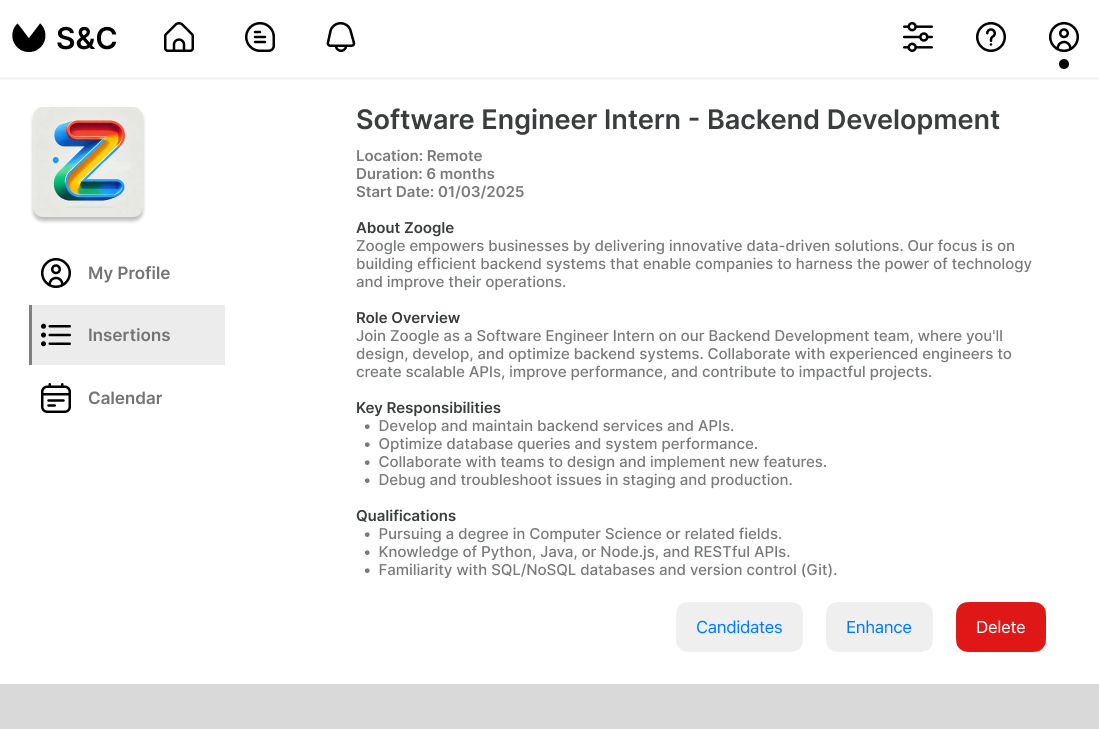
\includegraphics[width=0.75\linewidth]{DD/Images/UI/Insertions_selected.png}
    \caption{Insertion post example.}
    \label{fig:insertion_example_ui}
\end{figure}

\newpage

\textbf{\autoref{fig:insertion_candidates_ui}:} View Candidates

The third image shows the candidates associated with the selected insertion. The list includes:

\begin{itemize}
    \item 
Applied Candidates: Users who directly applied for the position.
    \item 
Recommended Candidates: Profiles suggested by the system based on a match with the insertion requirements.
\end{itemize}

Users can search candidates by name, and tabs allow switching between "Applied" and "Recommended."

\begin{figure}[H]
    \centering
    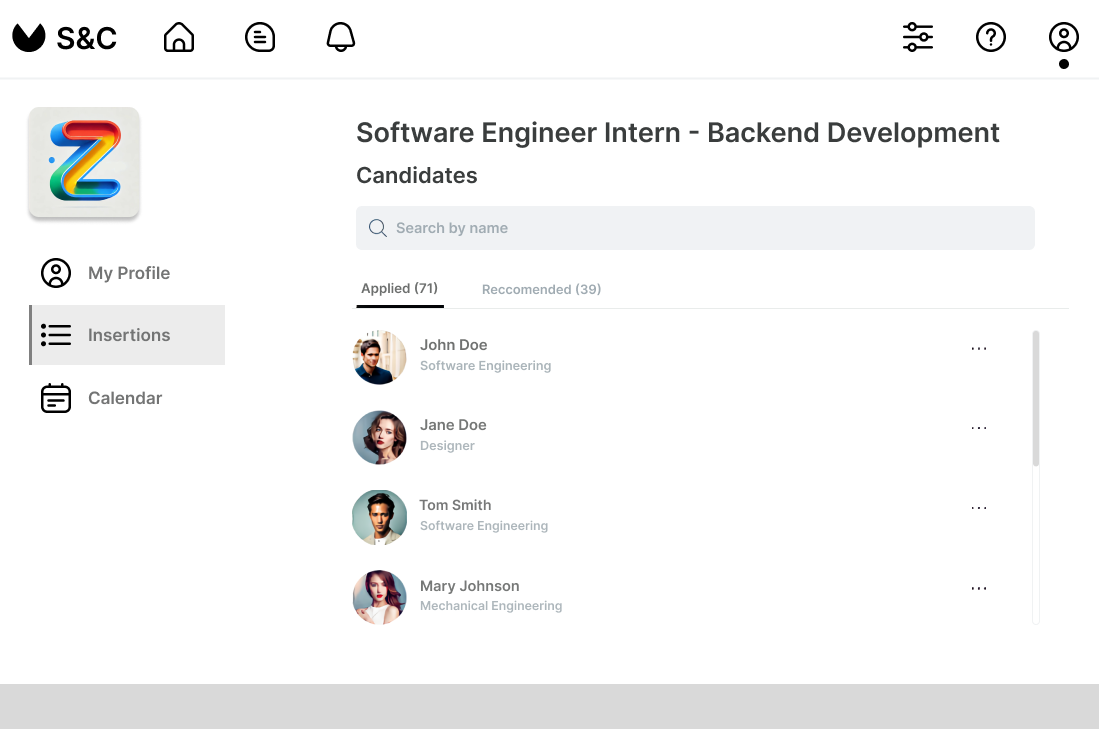
\includegraphics[width=0.75\linewidth]{DD/Images/UI/Insertions_selected_candidates.png}
    \caption{Insertion's candidates section.}
    \label{fig:insertion_candidates_ui}
\end{figure}

\newpage

\textbf{\autoref{fig:review_candidate_ui}:} Review and Accept a Candidate

In the last image, a specific candidate’s profile is opened (e.g., "John Doe"). The pop-up provides:

\begin{itemize}
    \item
Personal Information: City, date of birth, phone number.
    \item
Resume: A downloadable CV file.
\end{itemize}

And also two actions:

\begin{itemize}
    \item
Accept: Select the candidate and start a chat to proceed with further steps.
    \item 
Close: Exit the pop-up without taking action.
\end{itemize}

\begin{figure}[H]
    \centering
    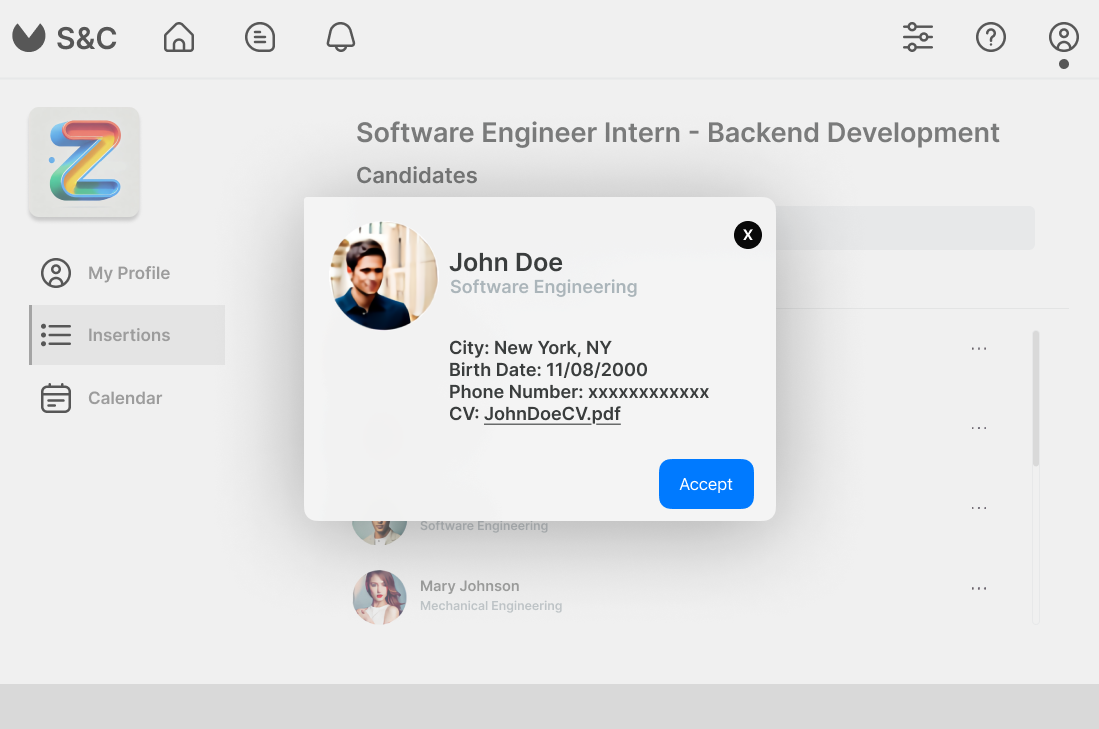
\includegraphics[width=0.75\linewidth]{DD/Images/UI/Insertions_selected_candidates_example.png}
    \caption{Review of a candidate.}
    \label{fig:review_candidate_ui}
\end{figure}

\newpage

\section{Schedule an Interview [UC14] and Start an Internship [UC15]}
\label{sec:UI6_interview_internship}%


\textbf{\autoref{fig:interview_proposal_ui}:} Interview Proposal
The first image represents a proposal for scheduling an interview. The company sends the interview details, including: position, location, time and date.
The student can either accept or decline through two buttons.

\begin{figure}[H]
    \centering
    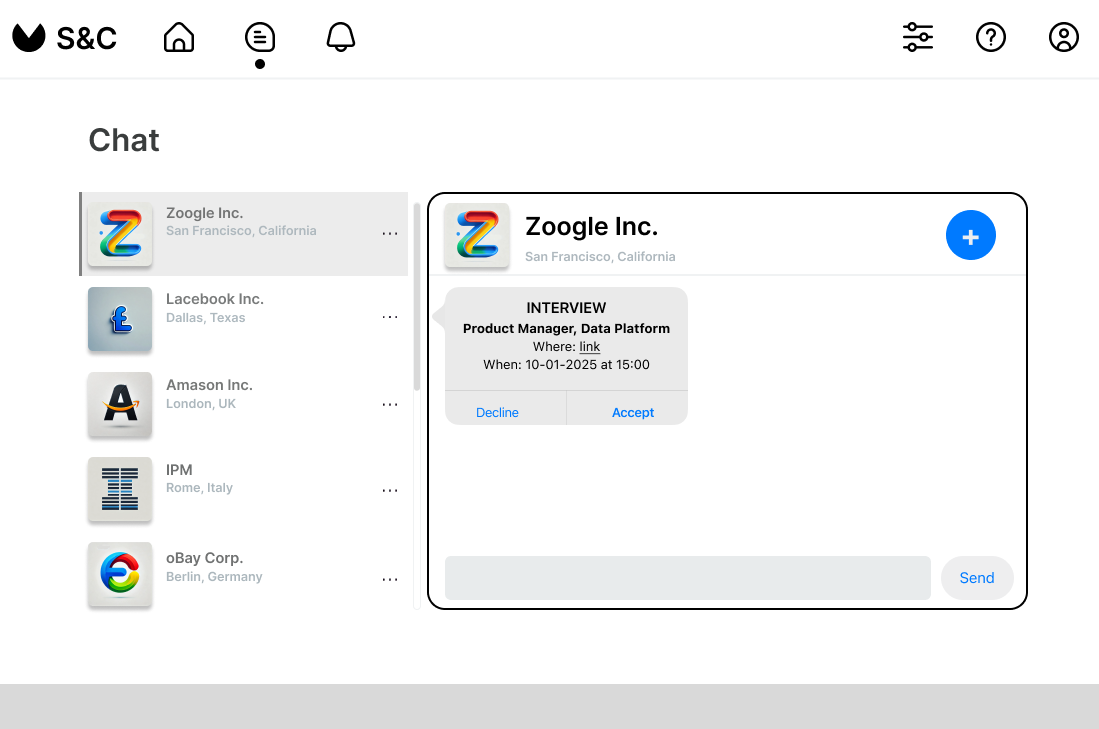
\includegraphics[width=0.75\linewidth]{DD/Images/UI/Chatpage_proposalInteview_student.png}
    \caption{Interview proposal.}
    \label{fig:interview_proposal_ui}
\end{figure}

\newpage

\textbf{\autoref{fig:internship_proposal_ui}:} Internship Proposal
The second image represents a proposal sent by a company (e.g., Zoogle Inc.) to a student in the chat. The proposal contains detailed information about the internship, such as: position, location, dates (start and end dates of the internship).
The student can either accept or decline through two buttons.

\begin{figure}[H]
    \centering
    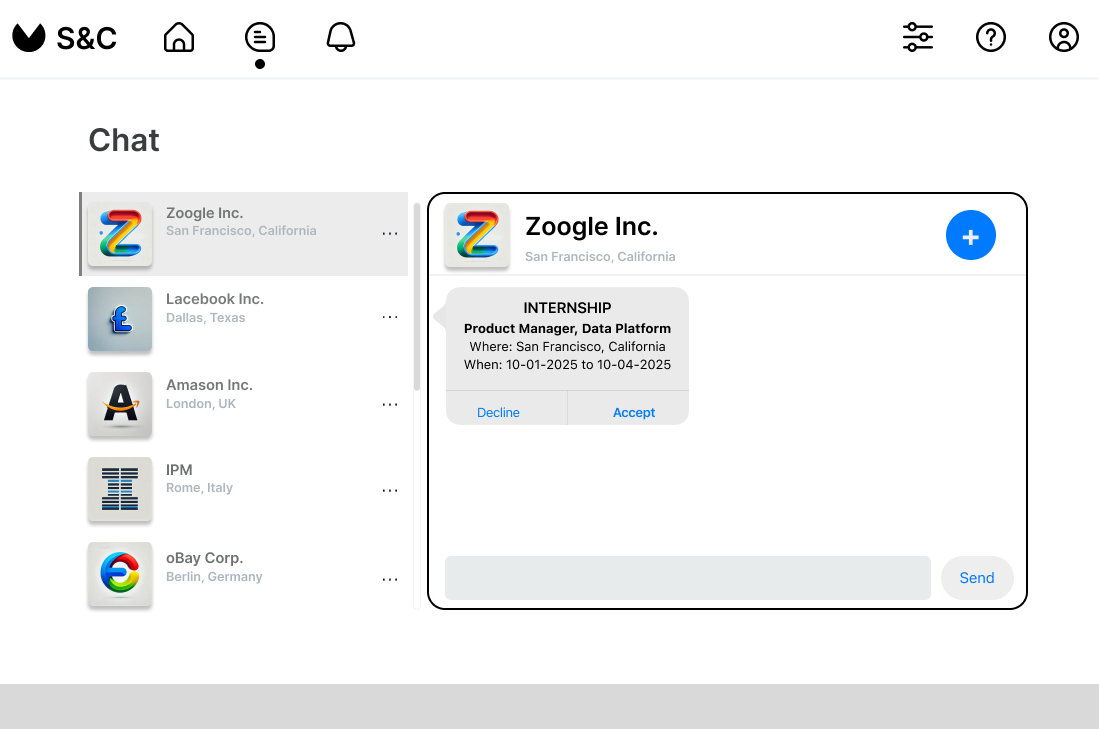
\includegraphics[width=0.75\linewidth]{DD/Images/UI/Chatpage_proposalInternship_student.png}
    \caption{Internship proposal.}
    \label{fig:internship_proposal_ui}
\end{figure}


\textbf{Interaction Flow}

In both cases, the chat serves as the main communication tool between the company and the student. The proposals allow quick and clear decisions, fostering seamless scheduling and internship acceptance processes. Once accepted, further discussions or confirmations can be carried out in the same chat interface.